\documentclass[11pt, a4paper, DIV=12]{scrartcl}

% useful packages 
\usepackage{mathtools}
\usepackage{physics}
\usepackage{graphicx}					  
\graphicspath{{figs/}}

\usepackage{amssymb}
\usepackage{amsmath}
\usepackage{hyperref}
\usepackage[separate-uncertainty=true]{siunitx}
\usepackage{xcolor}
\usepackage{braket} % easy braket notation
\usepackage{enumitem}
\usepackage{booktabs}
\usepackage{here}
\usepackage{cprotect}

\usepackage[backend=biber, sorting=none]{biblatex}
\bibliography{refs.bib}

% \numberwithin{equation}{section}

\title{ Multigrid simulation of the Gaussian model}
\date{\today}
\author{Harilal Bhattarai \& Marcel Schindler}
\begin{document}
	\maketitle
	
\section{Introduction}
In this exercise we want to apply the multigrid technique to the simulation of the Gaussian model in 1 dimension.
\section{Theory}
The microscopic degree of freedom is the real-valued field u with Hamiltonian given by,
\begin{equation}
	H_{\alpha}(u)=\frac{1}{a} \sum_{i=1}^{N}(u_{i}-u_{i-1})^{2}
\end{equation}
Where, a denotes the spacing between neighboring grid points and N = L/a.

The partition sum for the system is given by
\begin{equation}
	Z(\beta, N, a)= \prod_{i=1}^{N-1}\int_{- \infty}^{+ \infty}du_{i}(exp (-\beta H_{a}(u)))
\end{equation}
The magnetization is define as;
\begin{equation}
	m=\frac{a}{L}\sum_{i=1}^{N-1}u_{i}
	\label{equ:magnetization}
\end{equation} 
Where, the Fourier decomposition is $u_{l}=\sum_{i=1}^{N-1}c_{k} \sin(k\pi la/L)  $. Here $ c_{k} $ is the $ k^{th} $ Fourier coefficient.
 We need for the Hamiltonian on coarse levels the field $\phi^{(2a)}$ we derived the follwoing formula:
\begin{equation}
\phi^{(2a)}_i=(\phi^{(a)}_{2i-1}+2\phi^{(a)}_{2i}+\phi^{(a)}_{2i+1})/4+a^2(2\tilde{u}_{2i-1}-\tilde{u}_{2i-2}+\tilde{u}_{2i}-\tilde{u}_{2i+2}-\tilde{u}_{2i-3})
\end{equation}
We derived this by comparing the Hamilton on fine level and on coarse level.
\section{Analysis}
To determine the magnetization and energy after each sweep we have used Metropolis-Hastings accept/reject with the following algorithm:
\begin{itemize}
	\item choose a site x for update , $ x \sim U(1, \dots, N-1) $.
	\item propose new $ U_{0}(x)= U(x) +r\delta $ with $ r \sim U([-1, 1]) $ and $ \delta $ a fixed scale parameter.	
	\item Metropolis accept/reject N-1 times.
\end{itemize}
 Here we have plotted graph on the basis of equation \ref{equ:magnetization}. We got the output graphs of magnetization, square of magnetization and the energy as in figure \ref{fig:magnitization}. From our output graph \ref{fig:magnitization} we noticed that the magnetization oscillation has more wave numbers with small amplitude. Since no quite smooth waves. Here a small remark. We played a little bit with the random generator and got completly different results. We used one and got way to high values and $<m>$ was not even 0. Then We used one and got $<m>=0$ but with smaller values. We did not change the distribution. We only changed the random number generator. We have no idea what the right generator is which we can use in functions(We also had problems. That the generator did something different in the main function and in other functinos. Again we do not know exactly how these generators behave). For the analytic part we had not enought time because this cost a lot of time to get to the bottom of it. We know for sure that the $<m>=0$ because we have a simity in u, so it should not change with a sign because we take the square.

\begin{figure}[H]
	\centering
	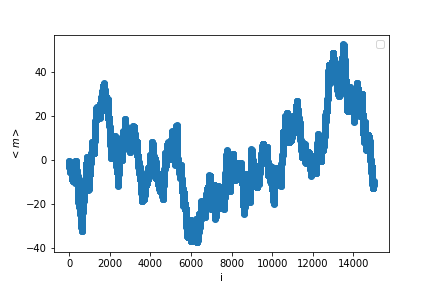
\includegraphics[width=0.6\linewidth]{magnitization.png}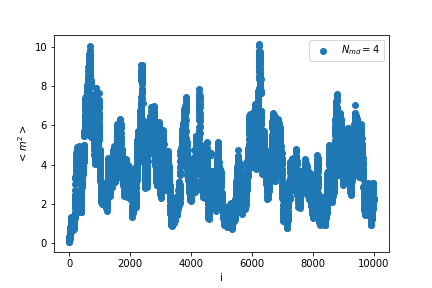
\includegraphics[width=0.6\linewidth]{magnitization_square.png}
	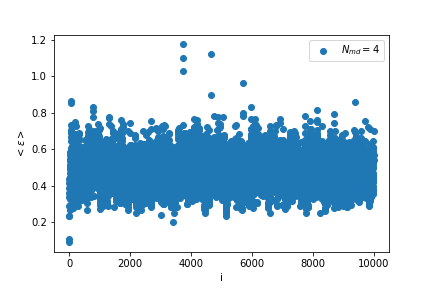
\includegraphics[width=0.8\linewidth]{energy.png}
	\caption{The distribution of magnetization, magnetization square and energy with i from 1 to (N-1) at $ N_{md}=4 $. Upper left graph for magnetization and right one is for square of magnetization and reaming one is for energy}
	\label{fig:magnitization}
\end{figure}

To plot autocorrelation function, we used the sampling with $ \delta=2 $, $ N=64 $ and $ \beta=1 $ and $n_{lvl}=3$. Moreover, we have set the number of sweeps for coarsest $ \nu_{pre}= \nu_{post}=4, 2, 1 $. Then we did two runs: V-cycle and W-cycle. That means at $ \gamma = $ 1 and 2. After that, we plotted the autocorrelation function of the squared magnetization as defined in equation \ref{equ:magnetization} using these two different cycles with these parameters. From the figure \ref{fig:autocorrelation} we see that that the autokorrelation goes faster to zero with $gamma=2$ and that there are still some ozillations. 
\begin{figure}[H]
	\centering
	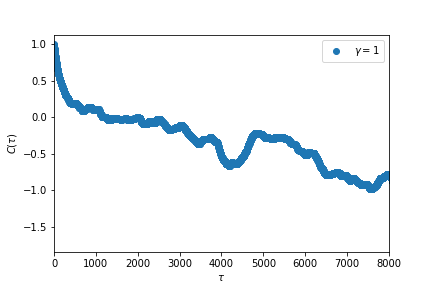
\includegraphics[width=0.6\linewidth]{magnitization_square_autocorrelation_gamma1.png}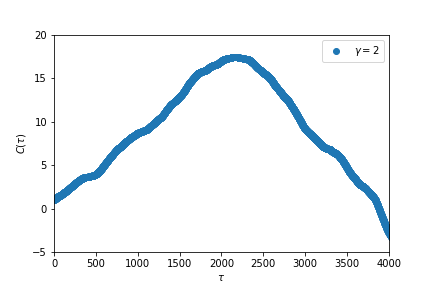
\includegraphics[width=0.6\linewidth]{magnitization_square_autocorrelation_gamma2.png}
	\caption{The magnetization square autocorrelation $\gamma =$ 1 and 2.}
	\label{fig:autocorrelation}
\end{figure}

Now we have used all ingredients to compile the multigrid simulation algorithm as in \cite{exercise-sheet} at the current level with spacing a. We get the magnetization square multigrid with $ \gamma = $ 1 and 2 as in figure \ref{fig:grid}. Again here a remark. If we look at the magnitization values, they are way to high but again we had not enought time to get to the bottom of it(Again we used different generators). We see that we have highly oszillation magnitization. which is not bad but the values are way to high.
\begin{figure}[H]
	\centering
	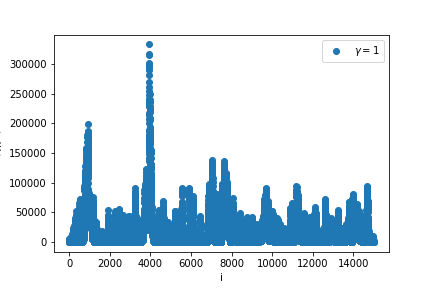
\includegraphics[width=0.6\linewidth]{magnitization_square_multigrid_gamma1.png}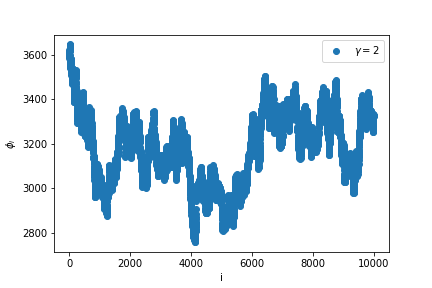
\includegraphics[width=0.6\linewidth]{magnitization_square_multigrid_gamma2.png}
	\caption{The magnetization square multi-grid $\gamma =$ 1 and 2.}
	\label{fig:grid}
\end{figure}



\section{Conclusion}
We saw in this weeks Problem how we can get the magnitization and energy with the multigrid formula. We again are not sure of our result. The autocorrelation function looks good, but for the magnitization we get to high values. For $<m>$ we get 0 which is what we expect. 
	
	
\begin{thebibliography}{12}
	\bibitem{exercise-sheet} 
	Thomas Luu, Andreas Nogga, Marcus Petschlies and  Andreas Wirzba, Exercise-sheet, 2020. 
\end{thebibliography}	
\end{document}	